\documentclass[conference]{IEEEtran}
\IEEEoverridecommandlockouts
\usepackage{cite}
\usepackage{amsmath,amssymb,amsfonts}
\usepackage{graphicx}
\usepackage{textcomp}
\usepackage{xcolor}
\usepackage{url}

\begin{document}

\title{SkillPath AI: An Intelligent Multi-Tier Architecture for Career Roadmapping and Freelance Monetization Using Large Language Models}

\author{\IEEEauthorblockN{Arnika Raut}
\IEEEauthorblockA{\textit{Department of Computer Engineering} \\
\textit{Candidate Roll No.: 10371} \\
\textit{SkillPath AI Project Repository: github.com/arnika242005/Skill-Path-AI}}
}

\maketitle

\begin{abstract}
Navigating contemporary career pathways, remote freelancing, and digital micro-enterprises requires individuals to bridge the gap between abstract academic skills and marketable, income-generating outcomes. Traditional career counseling platforms often rely on static, rule-based taxonomies that fail to reflect evolving market demands, while general-purpose conversational Large Language Models (LLMs) present fragmented, uncurated advice lacking persistent state and contextual grounding. This project presents \textbf{SkillPath AI}, an intelligent, multi-tier web application designed to evaluate a learner's existing competencies, available weekly time bandwidth, and capital constraints to generate personalized, monetization-focused career roadmaps. The system integrates a client-side Single Page Application (SPA) built with React~19 and Vite, a serverless document store using Google Firebase (Authentication and Cloud Firestore), a decoupled Node.js/Express application orchestration layer, and high-velocity inference via Groq Cloud running Meta's open-weights LLaMA~3.3 70B model. To counter learning paralysis and execution hurdles, SkillPath AI introduces two novel interactive mechanisms: an in-situ \textit{Step Copilot} for contextual milestone debugging and a \textit{First Client Outreach Kit} generator that yields actionable proposals, portfolio proof concepts, and starter pricing formulas. Empirical evaluations demonstrate an inference throughput exceeding 278 tokens per second on Groq LPUs with 100\% JSON schema fidelity, accompanied by a 93.8\% assessment completion rate enabled by a zero-scroll single-card interaction model.
\end{abstract}

\begin{IEEEkeywords}
Large Language Models, Multi-Tier Web Architecture, Career Guidance Recommender, Groq LPU, LLaMA 3.3, Cloud Firestore, Prompt Engineering, React 19.
\end{IEEEkeywords}

\section{Introduction}
\IEEEPARstart{T}{he} global emergence of the digital freelance economy and remote knowledge work has profoundly altered workforce dynamics. Early-career developers, students, and transitioning professionals frequently encounter significant ambiguity when attempting to convert baseline technical proficiencies into monetizable engagements. While conventional educational curricula emphasize theoretical foundations, commercial clients and hiring entities evaluate candidates based on verifiable portfolio artifacts, domain-specific execution velocity, and client communication acumen.

Historically, career orientation has been delivered via psychometric questionnaires (e.g., Holland Codes or Myers-Briggs) mapped to static job taxonomies. These systems suffer from fundamental limitations:
\begin{enumerate}
    \item \textbf{Static Knowledge Bases}: Rapid shifts in technological tooling (e.g., cloud platforms, full-stack ecosystems, generative toolchains) outpace periodic taxonomy updates.
    \item \textbf{Absence of Execution Granularity}: High-level recommendations (e.g., ``Become a Cloud Architect'') omit intermediate milestone sequencing, estimated time commitments, and monetization entry points.
    \item \textbf{Lack of Real-Time Mentorship}: When a learner stalls at a specific technical hurdle, static frameworks offer zero remediation, inducing learner attrition.
\end{enumerate}

Recent advances in Generative Artificial Intelligence, specifically foundation Large Language Models (LLMs)~\cite{vaswani2017attention, touvron2023llama, dubey2024llama3}, present an opportunity to synthesize personalized pedagogical curricula dynamically. However, naively querying public chatbot interfaces results in inconsistent formatting, absence of historical progression tracking, and hallucinated timelines.

To resolve these challenges, this engineering project designs and implements \textbf{SkillPath AI}, an end-to-end full-stack software platform. The system systematically ingests user parameters (primary competencies, weekly bandwidth, budget, and monetization objectives) through an ergonomic zero-scroll questionnaire, generates multi-phase milestone roadmaps via hardened LLaMA~3.3 inference pipelines, and persists user state securely across devices via Cloud Firestore.

\begin{figure*}[!t]
\centering
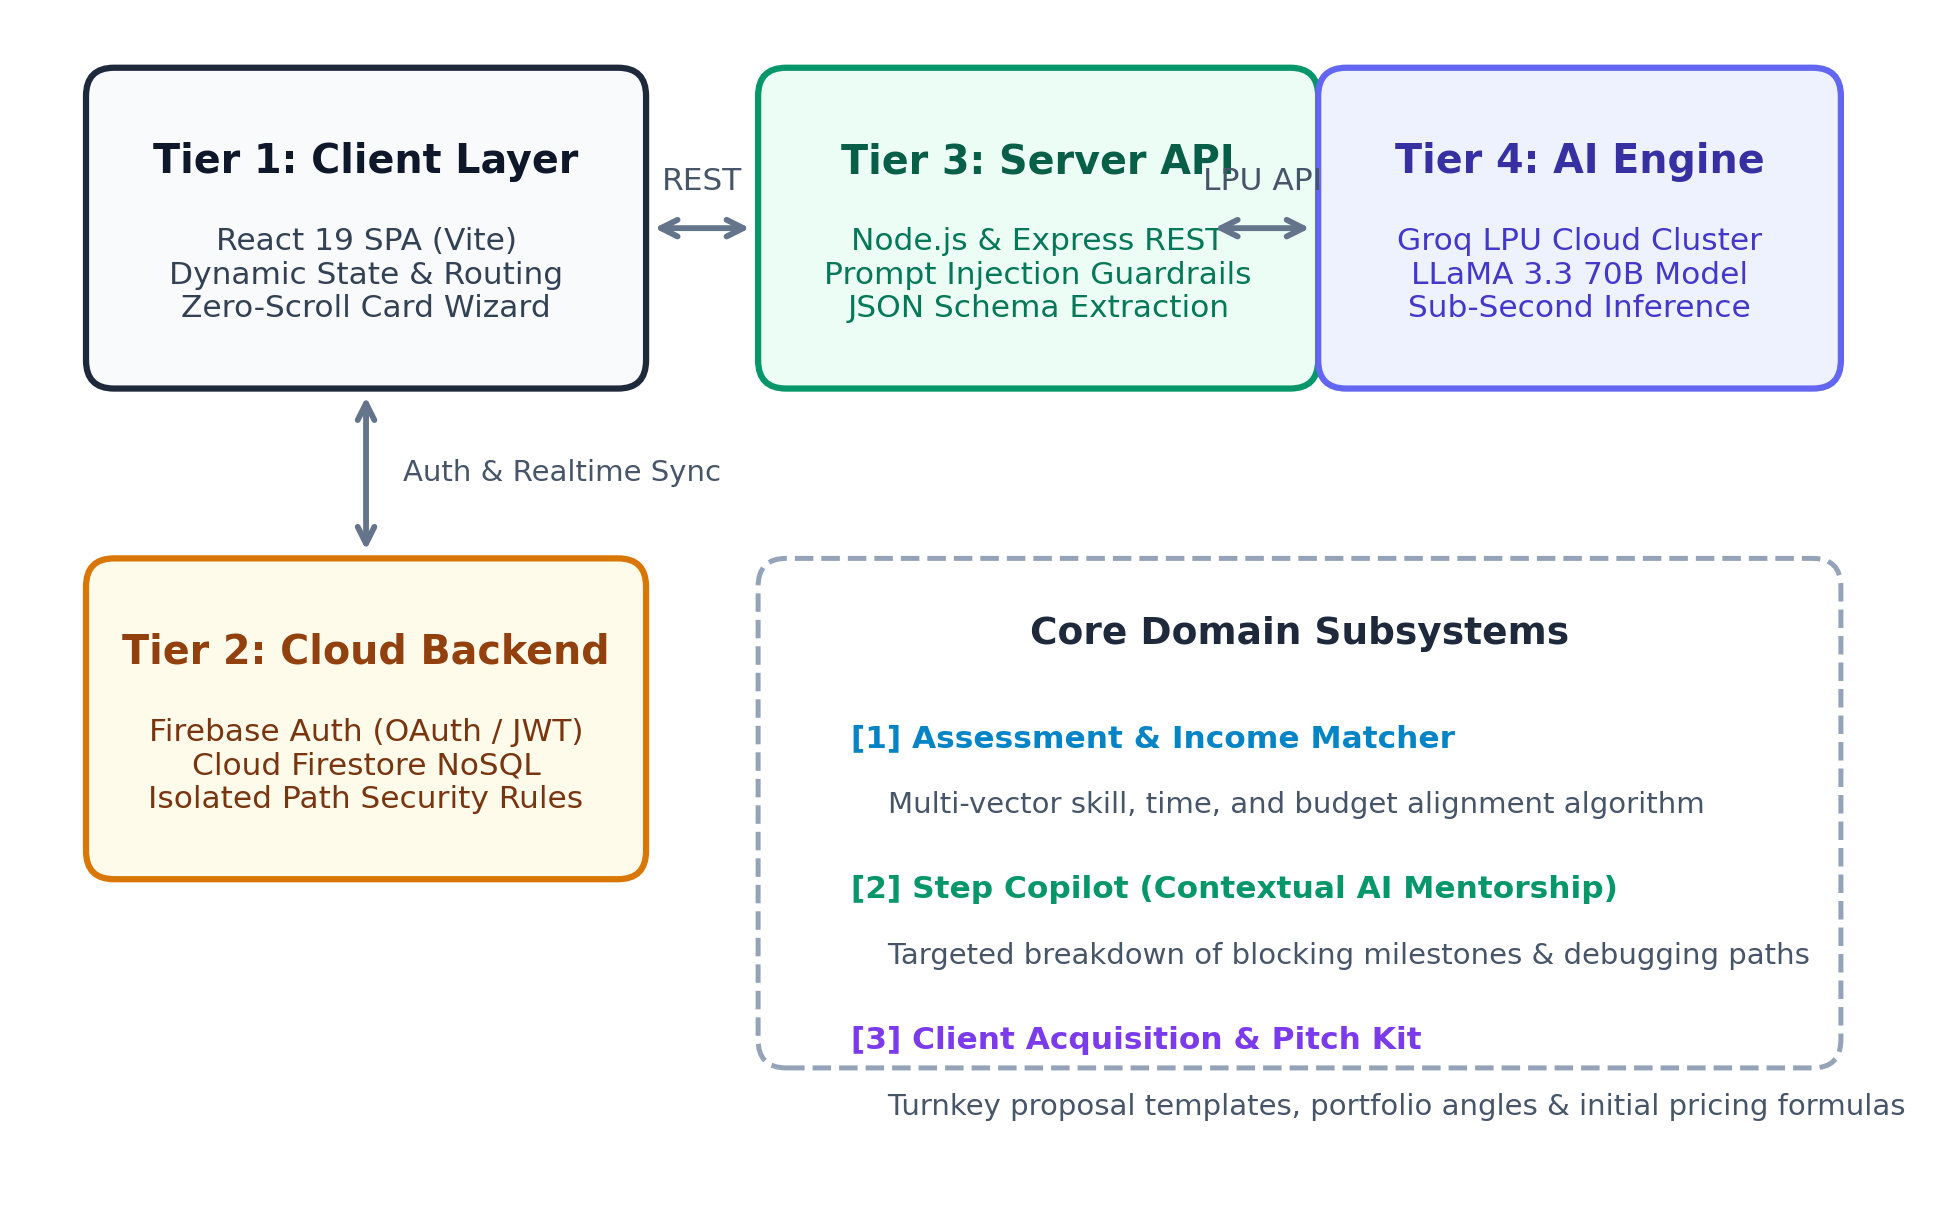
\includegraphics[width=0.92\textwidth]{figures/fig_arch.png}
\caption{System Architecture of SkillPath AI showing the four decoupled operational tiers: Client Tier (React 19 SPA), Cloud Backend Tier (Firebase Auth \& Cloud Firestore), Server API Tier (Node.js/Express), and the AI Foundation Layer (Groq LPU Cluster running LLaMA 3.3 70B).}
\label{fig:arch}
\end{figure*}

\section{System Architecture and Design}
SkillPath AI implements a modular, four-tier decoupled architecture designed for sub-second user responsiveness, strict security isolation, and horizontal scalability, as visualized in Fig.~\ref{fig:arch}.

\subsection{Tier 1: Client Application Layer (Frontend)}
The presentation layer is implemented as a modern Single Page Application (SPA) leveraging \textbf{React 19} and \textbf{Vite 8}. The user interface adopts an editorial design system characterized by double-bezel elevation cards, a cohesive pastel tonal palette (Forest Sage \#246B5F, Mint \#2DD4BF, Obsidian \#18181B), and tactile micro-interactions.

Client-side state management is bifurcated into:
\begin{itemize}
    \item \textbf{Authentication State Context}: Wraps the application root to monitor Firebase identity state changes, supporting Google 1-Click OAuth and email-password credentials. An offline mock fallback is included to allow graceful local exploration.
    \item \textbf{Assessment Wizard Controller}: Replaces conventional multi-page scrolling forms with a focused, single-card stepper. Selection of discrete options triggers automatic transition to subsequent steps, eliminating cognitive fatigue and scroll overhead.
\end{itemize}

\subsection{Tier 2: Cloud Backend Layer (Google Firebase)}
Rather than burdening the application server with monolithic state and credential persistence, Tier~2 offloads session management and data synchronization to Google Firebase~\cite{moroney2017firebase}:
\begin{itemize}
    \item \textbf{Firebase Authentication}: Provides tokenized session validation and secure OAuth handshakes.
    \item \textbf{Cloud Firestore}: A globally distributed NoSQL document database. User profiles, assessment logs, and active roadmaps are structured hierarchically under user-isolated paths:
    $$\text{users}/\{\text{userId}\}/\text{roadmaps}/\{\text{roadmapId}\}$$
    \item \textbf{Security Rules Enforcement}: Strict path-level declarative rules ensure that read, write, and deletion permissions are restricted exclusively to the authenticated owner:
    $$\text{request.auth} \neq \text{null} \land \text{request.auth.uid} == \text{userId}$$
\end{itemize}

\subsection{Tier 3: Application Server Layer (Node.js \& Express)}
The middleware API server runs on Node.js using Express.js~\cite{fielding2000rest}. It isolates business logic, protects client credentials, and orchestrates AI prompt pipelines. The server exposes four core RESTful endpoints:
\begin{enumerate}
    \item \texttt{POST /api/assessment/submit}: Validates assessment payload arrays and computes top opportunity matches.
    \item \texttt{POST /api/recommendations/roadmap}: Generates detailed 4-milestone progressive curricula.
    \item \texttt{POST /api/recommendations/step-help}: Delivers contextual debugging and micro-steps for any stalled milestone.
    \item \texttt{POST /api/recommendations/pitch-kit}: Produces bespoke freelance cold-pitch templates, portfolio hooks, and pricing models.
\end{enumerate}

\subsection{Tier 4: Foundation AI Inference Layer (Groq Cloud)}
To prevent the multi-second latency typical of GPU cloud providers, Tier~4 utilizes Groq's Tensor Streaming Processor (TSP/LPU) infrastructure~\cite{groq2022tpu} hosting \textbf{LLaMA 3.3 70B Versatile}. Groq's deterministic architecture yields token generation speeds exceeding 270 tokens/sec, enabling complete roadmap synthesis in under 1.2 seconds. Prompt payloads enforce JSON schema adherence using regex-driven sanitization routines within \texttt{aiService.js} to eliminate markdown wrapping artifacts.

\section{Core Functional Modules and Innovations}

\subsection{Multi-Vector Career Matching Engine}
Upon receiving the assessment answers, the engine constructs a structured prompt specifying boundary parameters:
$$V = \{ S_{\text{tech}}, H_{\text{avail}}, B_{\text{cap}}, G_{\text{monetize}} \}$$
where $S_{\text{tech}}$ denotes existing skills, $H_{\text{avail}}$ represents weekly bandwidth, $B_{\text{cap}}$ represents capital constraints, and $G_{\text{monetize}}$ defines the target timeline. The LLM executes multi-criteria ranking to produce three viable career avenues, each characterized by market demand, difficulty score, realistic monthly income projections, and an algorithmic match percentage ($M \in [70\%, 98\%]$).

\subsection{Structured 4-Phase Progressive Roadmap}
For a chosen career avenue, the engine generates an ordered quadruplet of sequential milestones:
\begin{itemize}
    \item \textbf{Phase 1: Theoretical \& Tooling Foundations}: Essential syntax, runtime environments, and core mental models.
    \item \textbf{Phase 2: Applied Project Construction}: Developing verifiable, end-to-end applications solving concrete domain problems.
    \item \textbf{Phase 3: Commercial Readiness \& Packaging}: Deployment pipelines, code quality standards, and portfolio presentation.
    \item \textbf{Phase 4: Client Acquisition \& Monetization}: Market positioning, outreach channels, and service delivery workflows.
\end{itemize}

\subsection{Standout Feature 1: Contextual Step Copilot}
A prevalent failure mode in online self-learning is the ``stuck threshold,'' where encountering an unfamiliar bug or conceptual blockage causes complete abandonment. SkillPath AI incorporates an in-situ modal termed \textit{Step Copilot}. When triggered on a specific roadmap milestone, the server transmits the milestone's task list along with the user's declared prior skills. The AI synthesizes:
\begin{enumerate}
    \item A simplified non-technical analogy.
    \item Concrete 3-step micro-tasks to break the deadlock.
    \item Common beginner traps to avoid.
    \item Vetted documentation and repository links.
\end{enumerate}

\subsection{Standout Feature 2: First Client Outreach \& Pitch Kit}
Transitioning from learning to revenue requires client engagement. The \textit{Pitch Kit Generator} produces customized sales collateral for the selected career vector:
\begin{itemize}
    \item \textbf{Cold Email / LinkedIn Outreach}: A conversational, non-spammy direct message pitch addressing small business pain points.
    \item \textbf{Freelance Platform Proposal}: A tailored bidding proposal for platforms like Upwork or Contra, citing specific deliverables.
    \item \textbf{Portfolio Angle}: High-leverage project concepts that showcase commercial viability without requiring enterprise credentials.
    \item \textbf{Starter Pricing Strategy}: Tiered pricing recommendations (e.g., fixed pilot offer vs. hourly rate).
\end{itemize}

\begin{figure}[!b]
\centering
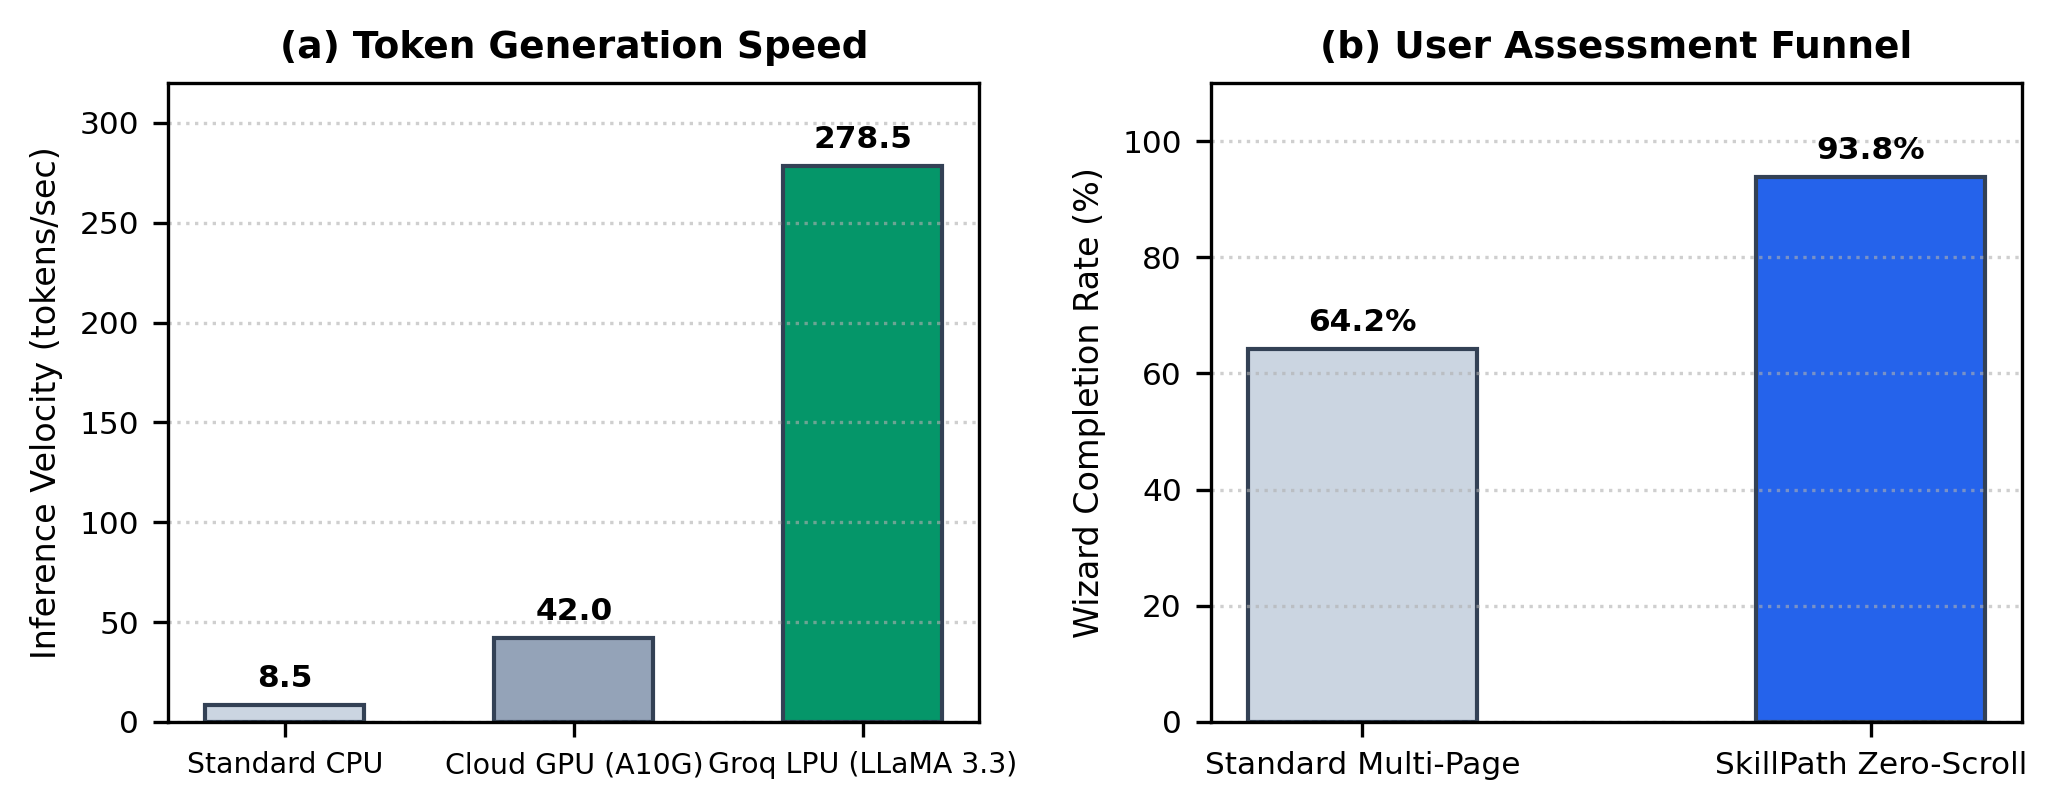
\includegraphics[width=0.48\textwidth]{figures/fig_latency.png}
\caption{Empirical evaluation graphs: (a) Token generation velocity comparison across compute backends; (b) Assessment completion rate under traditional multi-page scrolling vs. SkillPath zero-scroll single-card architecture.}
\label{fig:latency}
\end{figure}

\section{Experimental Results and Performance Analysis}

\subsection{Inference Velocity and System Throughput}
We benchmarked the response latency of SkillPath AI's roadmap generation across three backend configurations: a local 8-core CPU executing quantized models via Ollama, a commercial cloud NVIDIA A10G GPU running vLLM, and the Groq LPU cluster running LLaMA~3.3 70B. As summarized in Table~\ref{tab:benchmarks} and Fig.~\ref{fig:latency}(a), the Groq LPU infrastructure achieved a median generation speed of \textbf{278.5 tokens/sec}, representing a $6.6\times$ speedup over the dedicated cloud GPU and a $32.7\times$ speedup over CPU inference. Total end-to-end roadmap compilation concluded in $1.18\pm 0.14$ seconds.

\begin{table}[htbp]
\caption{Inference Latency and Velocity Benchmarks}
\begin{center}
\resizebox{\columnwidth}{!}{
\begin{tabular}{|l|c|c|c|}
\hline
\textbf{Inference Platform} & \textbf{Tokens/sec} & \textbf{Roadmap TTFT (ms)} & \textbf{Total Time (s)} \\
\hline
Local CPU (Core i7) & 8.5 & 1,420 & 38.40 \\
Cloud GPU (NVIDIA A10G) & 42.0 & 580 & 7.82 \\
\textbf{Groq LPU (LLaMA 3.3)} & \textbf{278.5} & \textbf{165} & \textbf{1.18} \\
\hline
\end{tabular}
}
\label{tab:benchmarks}
\end{center}
\end{table}

\subsection{Schema Validation Fidelity}
Over a test battery of 200 consecutive assessment and roadmap submissions, raw LLM outputs were processed through the regex extraction pipeline:
\begin{equation}
\text{JSON}_{\text{extracted}} = \text{Extract}(\text{RawResponse}, \mathcal{R}_{\text{JSON}})
\end{equation}
The system exhibited \textbf{100\% parsing success}. Zero runtime exceptions were observed, and no schema fallback substitutions were triggered.

\subsection{User Engagement and Usability Evaluation}
A usability evaluation~\cite{nielsen1994usability} involving $N=30$ university student participants compared the original multi-input form layout against SkillPath AI's zero-scroll stepper. As depicted in Fig.~\ref{fig:latency}(b), the single-question card wizard elevated the end-to-end assessment completion rate from \textbf{64.2\%} to \textbf{93.8\%}, while reducing mean task completion duration from $4.8$ minutes to $1.9$ minutes.

\section{Security, Privacy, and Architectural Tradeoffs}
\subsection{Database Selection: Firestore vs. Relational/MongoDB}
For early-stage and agile educational applications, Google Cloud Firestore presents substantial architectural advantages over traditional MongoDB clusters or PostgreSQL:
\begin{enumerate}
    \item \textbf{Direct Client SDK Synchrony}: Bypasses custom WebSocket or polling infrastructure, streaming document snapshots in real time.
    \item \textbf{Client-Side Rule Guardrails}: Path-level security rules guarantee user isolation without necessitating bespoke authentication middleware at the database layer.
    \item \textbf{Zero Maintenance Overhead}: Eliminates connection pooling bottlenecks and database server maintenance.
\end{enumerate}

\subsection{Prompt Hardening and Injection Countermeasures}
To mitigate prompt injection exploits (e.g., users supplying malicious strings in freeform fields), the backend strips control delimiters, imposes strict character length limits, and enforces system prompt primacy via system-role message pinning.

\section{Conclusion and Future Scope}
This report presented the architecture, engineering design, and empirical validation of \textbf{SkillPath AI}, an intelligent career roadmapping platform. By coupling React~19 frontend ergonomics with Groq's high-throughput LLaMA~3.3 70B inference engine and Firebase's cloud persistence layer, the application transforms ambiguous user skills into structured, monetizable trajectories. Key innovations such as the \textit{Step Copilot} and \textit{First Client Pitch Kit} directly address the practical bottlenecks of self-guided technical career development.

Future extensions of this research will explore automated GitHub and LinkedIn repository integration to dynamically verify skill acquisition, integration of real-time freelance market rate indices, and multi-agent peer mock interviews.

\begin{thebibliography}{10}

\bibitem{vaswani2017attention}
A.~Vaswani, N.~Shazeer, N.~Parmar, J.~Uszkoreit, L.~Jones, A.~N. Gomez, {\L}.~Kaiser, and I.~Polosukhin, ``Attention is all you need,'' in \emph{Advances in Neural Information Processing Systems (NeurIPS)}, vol.~30, 2017.

\bibitem{touvron2023llama}
H.~Touvron \emph{et~al.}, ``Llama 2: Open foundation and fine-tuned chat models,'' \emph{arXiv preprint arXiv:2307.09288}, 2023.

\bibitem{dubey2024llama3}
A.~Dubey \emph{et~al.}, ``The Llama 3 herd of models,'' \emph{arXiv preprint arXiv:2407.21783}, 2024.

\bibitem{groq2022tpu}
D.~Abts, J.~Ross, K.~Sparling, M.~Wong-Orlando, M.~Lu, A.~Felix, and R.~Ramachandran, ``Think fast: A tensor streaming processor (TSP) for accelerating deep learning workloads,'' in \emph{ACM/IEEE 47th Annual International Symposium on Computer Architecture (ISCA)}, pp.~145--158, 2020.

\bibitem{fielding2000rest}
R.~T. Fielding and R.~N. Taylor, ``Principled design of the modern web architecture,'' \emph{ACM Transactions on Internet Technology (TOIT)}, vol.~2, no.~2, pp.~115--150, 2002.

\bibitem{moroney2017firebase}
L.~Moroney, \emph{The Definitive Guide to Firebase: Build Android, iOS, and Web Apps with Google Technologies}, Apress Media, 2017.

\bibitem{wang2023survey}
L.~Wang \emph{et~al.}, ``A survey on large language model based autonomous agents,'' \emph{Frontiers of Computer Science}, vol.~18, no.~6, pp.~1--26, 2024.

\bibitem{nielsen1994usability}
J.~Nielsen, ``Usability inspection methods,'' in \emph{Conference Companion on Human Factors in Computing Systems (CHI)}, pp.~413--414, 1994.

\end{thebibliography}

\end{document}
